
%===================================================================================================
%===================================================================================================
\section{{\torchgpipe}: A PyTorch Library for GPipe}
\label{sec:torchgpipe}
%===================================================================================================
%===================================================================================================

{\torchgpipe} is a PyTorch library for micro-batch pipeline parallelism with checkpointing, as known as GPipe. The library provides a simple way to apply GPipe to a generic sequential module written in PyTorch. The usage of {\torchgpipe} resembles that of the data parallel module of PyTorch --- just wrap your model with the wrapper.

Users must specify the number of micro-batches $m$ and how consecutive layers form $n$ partitions. Here we remark that even though we simplified our assumption to that the model is a sequence of partitions, it is strictly required in {\torchgpipe} that the model is a sequence of \emph{layers} to give flexibility for users how to split the model. {\torchgpipe} will assume that each layer is a non-divisible, black-box, and referentially transparent\footnote{This is required especially for checkpointing: referential transparency ensures that recomputation is identical to the computation done in the forward pass.} algorithm. 

For convenience, the library provides the submodule \cmtt{torchgpipe.balance} which computes a partition whose pairwise resource discrepancy is small, where resource consumption is computed by profiling. Specifically, we used the algorithm from \cite{barany2015block}.

As {\torchgpipe} is built on PyTorch equipped with CUDA backend, we will often assume that devices are NVIDIA GPU throughout this section. Nevertheless, the underlying principle of the library applies in general for implementing pipeline parallelism any eager execution environments.


%===================================================================================================
\subsection{Complications in PyTorch}
\label{subsec:obstacles}
Our primary concern is efficiency. As we discussed in \autoref{subsec:timeline}, in order for pipeline parallelism to work as desired, the tasks must be assigned to each device in the correct order. There are several complications to achieve this in PyTorch. 

First of all, kernels are issued to each device on-the-fly due to PyTorch's define-by-run style and its eager execution behavior (as opposed to in construct-and-run type frameworks). Hence, one must design the host code carefully so not only that device-bound tasks are issued in the correct order within each device, but also that execution of the tasks on devices (asynchronous to CPU) are not delayed due to the Python interpreter failing to request it ahead of the time. This kind of delay may happen when some of the tasks are CPU-intensive or involve a lot of cheap kernel calls. As a solution, {\torchgpipe} introduces deterministic clock-cycle which gives the total ordering of the tasks.

Secondly, the computation graph for backward pass is constructed dynamically during the forward pass in PyTorch. In other words, \emph{``it avoids ever materializing a ``forward graph'', recording only what is necessary to differentiate the computation.''} \cite{paszke2017automatic} Since PyTorch does not record the forward computation graph nor maintain a gradient tape, the automatic differentiation (autograd) engine of PyTorch does back-propagation solely with respect to the graph. It implies that autograd engine may not run exactly in the reverse order of execution as in the forward pass, unless enforced by the structure of the graph. To deal with this, we develop a pair of primitive functions called `fork' and `join' to create explicit dependencies on the fly in the backward computation graph.

Thirdly, communication between several devices can cause two-way synchronization, if not carefully managed. This may cause under-utilization since sender may wait to synchronize with the receiver even when there is no explicit dependency between the copy and next task in queue, or vice versa. {\torchgpipe} avoids this issue by using non-default CUDA streams so that copies would never block computations unless the computation must wait for the data.


Lastly, {\torchgpipe} attempts to relax the restriction of micro-batch pipeline parallelism that model must be sequential. Although any neural network can be written in a sequential form in principle, this requires knowing the entire computation graph ahead of the time which is not the case in PyTorch. In particular, if there is a tensor which skips from a layer in device $j'$ to another layer in device $j > j'+1$, the tensor will be copied to all devices in between since {\torchgpipe} cannot know it ahead.
To circumvent this issue, we design an interface to signify which intermediate tensors are skipped and which layers use them.


%===================================================================================================
\subsection{Optimization Components}
\label{subsec:implementation}
In the remainder of this section, it is explained how the components of {\torchgpipe} are designed and why each of them is essential for performance.

\subsubsection{Forward Dependency: Deterministic Clock-cycle}
\label{subsubsec:deterministic-clock-cycle}
As we discussed in \autoref{subsec:obstacles}, the total ordering of tasks is determined by the host code in the forward pass. Each device implicitly understands the dependency between tasks by the order they are assigned by CPU. Ideally, if tasks could be assigned to devices with no cost, CPU may assign tasks to devices in any order as long as the ordering within device is correct. However, this assumption is not realistic enough, as launching kernels on a GPU is not free for CPU, memory transfer between GPUs may require synchronization, or a task is CPU-intensive. For this reason, we minimize the delay coming from CPU by sorting all tasks by the distance to $F_{1,1}$.

\begin{algorithm}
\For{$k$ from $1$ to $m+n-1$}{
    \For{$i, j$ such that $i + j - 1 = k$}{
        \If{$j > 1$}{
            Copy $x_i^{j-1}$ to device $j$.
        }
    }
    \For{$i, j$ such that $i + j - 1 = k$}{
        Execute $F_{i,j}$.
    }
}
\caption{Deterministic clock-cycle}
\label{alg:clock-cycle}
\end{algorithm}

We call this \emph{deterministic clock-cycle} (\autoref{alg:clock-cycle}). In the algorithm, CPU executes the clock cycles starting from the counter $k=1$ to $k=m+n-1$. In $k$th clock cycle, all copy kernels for data needed to execute tasks $F_{i,j}$ where $i+j-1=k$ are first issued, and then the computation kernels for executing the tasks are registered to corresponding devices (which can be safely multithreaded since tasks in the same clock cycle are independent). 


\subsubsection{Backward Dependency: Fork and Join}
\label{subsubsec:fork-join}

\begin{figure}
\center
    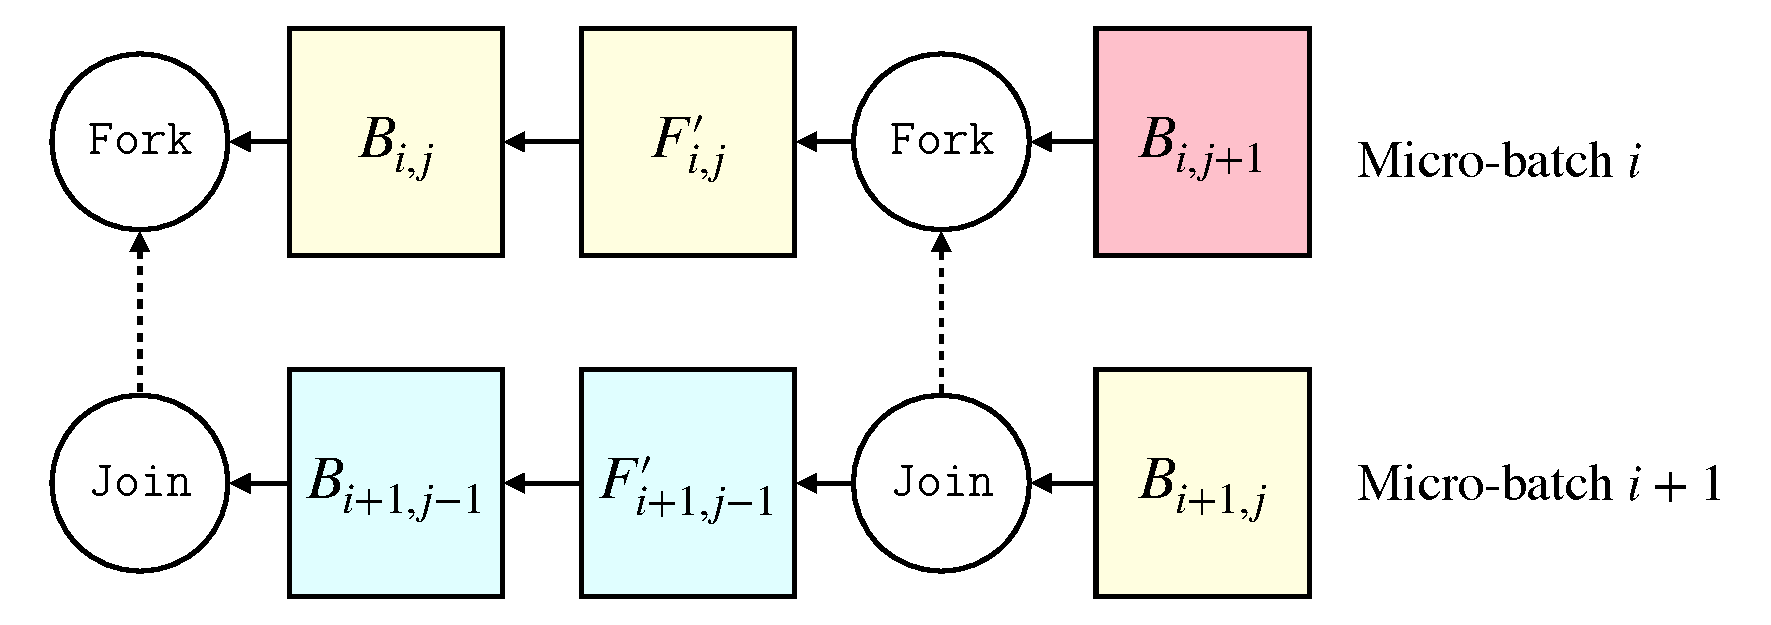
\includegraphics[width=0.5\textwidth]{figures/fork-and-join.pdf}
    \caption{The backward computation graph with \cmtt{Fork} and \cmtt{Join}. Different colors correspond to different devices. Arrows are drawn according to the \emph{direction in backward computation graph} and these relations are constructed during the forward pass. Here the virtual depedency of $F_{i,j}'$ on $B_{i+1, j}$ is created via \cmtt{Fork} and \cmtt{Join}, which is illustrated by dashed arrows.}
    \label{fig:fork-and-join}
\end{figure}

Suppose now that we run a forward pass according to the deterministic clock-cycle. The resulting computation graph for backward will look rather like \ref{fig:dependency} than \ref{fig:pp-with-checkpointing}, even when the forward tasks $F_{1,j},\cdots,F_{m,j}$ on device $j$ were executed in order. From such a graph, autograd engine of PyTorch would never know that $B_{i+1, j}$ must be executed before $B_{i, j}$, and this messes up the timeline of the backward pass. For this reason, virtual dependencies (dashed arrows in \autoref{fig:pp-with-checkpointing}) must be explicitly drawn during the forward pass.

We design a pair of primitive functions called \cmtt{Fork} and \cmtt{Join} to express such dependency. Basically, \cmtt{Fork} is the autograd function mapping a tensor $x$ to the pair $(x, \varnothing)$ where $\varnothing$ is an empty tensor\footnote{In principle, the tensor which indicates the virtual dependency can be arbitrary. We chose to use the empty tensor for this, however, to remove any unnecessary computation caused by the tensor such as gradient accumulation in PyTorch.}, and \cmtt{Join} is the autograd function mapping a pair $(x, \varnothing)$ to the tensor $x$. Now, dependency of $F_{i+1, j}$ upon $F_{i, j}$ (which translates to the dependency of $B_{i, j}$ upon $B_{i+1, j}$ in the backward computation graph) can be expressed as
\[
\begin{aligned}
( x_i^j, \varnothing ) &\ot \text{\cmtt{Fork}}(x_i^j) \\
x_{i+1}^{j-1} &\ot \text{\cmtt{Join}}( x_{i+1}^{j-1}, \varnothing ).
\end{aligned}
\]
See \autoref{fig:fork-and-join} for illustration.

\begin{figure*}[b]
\center
    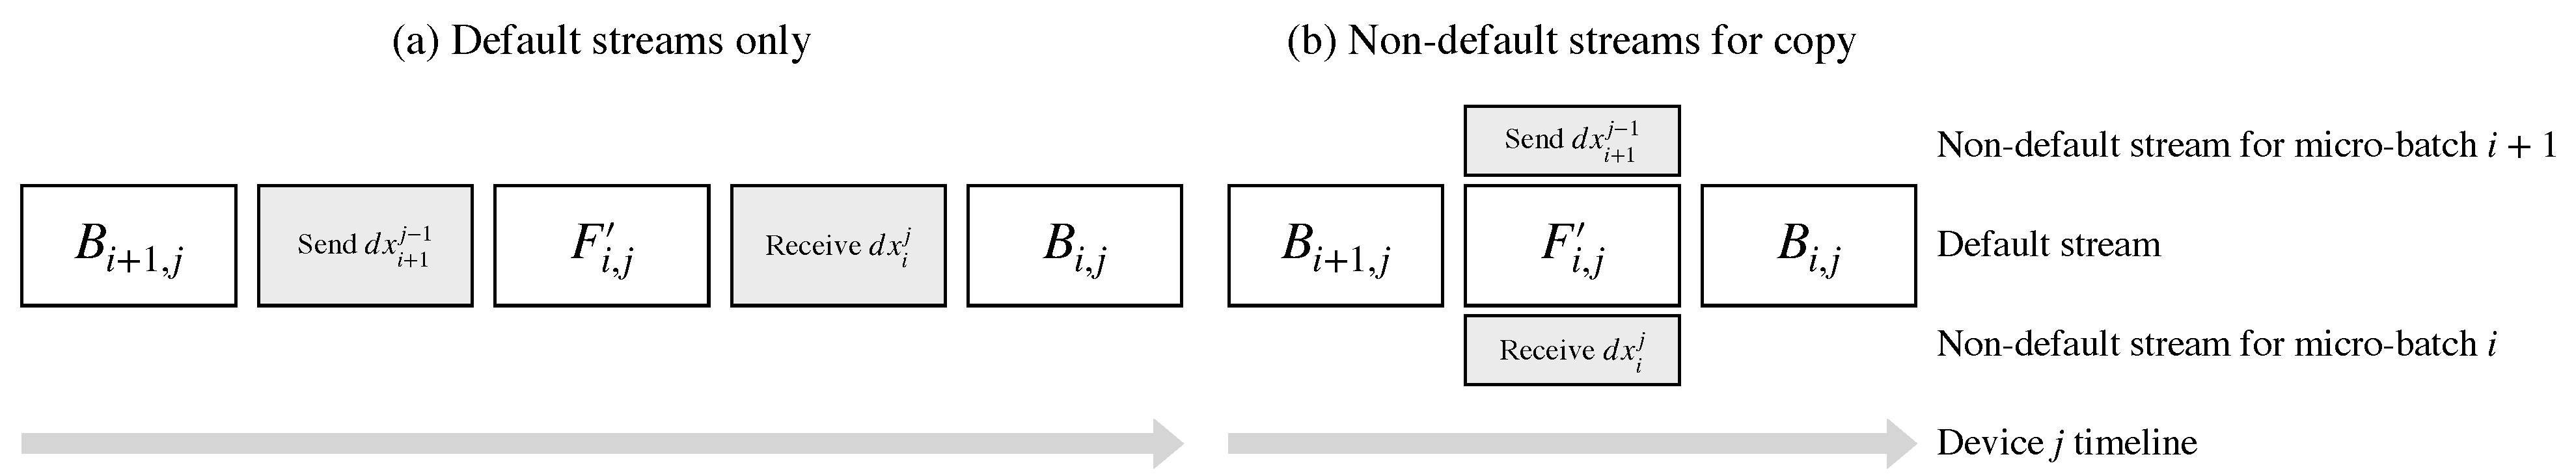
\includegraphics[width=\textwidth]{figures/copy-streams.pdf}
    \caption{Timeline of device $j$ with or without non-default streams for copy. (a): If only default streams are used, copy kernels may block computation kernels (and vice versa) until the copy is completely finished. (b): With copy streams, computation can happen in concurrent with sending or receiving data from other devices.}
    \label{fig:copy-streams}
\end{figure*}

\subsubsection{Concurrent Copy and Computation: Streams}
\label{subsubsec:copy-streams}

PyTorch issues every device-bound kernels to the default stream, unless it is specified otherwise. Stream is a device-bound sequence of kernels that is executed in order. Kernels in the same stream are guaranteed to be executed in the prescribed order, but kernels in different streams can be interleaved, and even can overlap when possible. In particular, nearly all CUDA devices with compute capability 1.1 and higher support concurrent copy and execution: data transfer between devices can always overlap with kernel execution (see section 4.5.1.5 of \cite{nvidia2007cuda}).

{\torchgpipe} registers every copy kernel to non-default streams while keeping computation kernels on the default stream. This allows the device $j$ processing $F_{i, j}$ in concurrent with sending $x_{i-1}^j$ to the device $j+1$ and/or receiving $x_{i}^{j-1}$ from the device $j-1$. Moreover, each device uses different streams for each micro-batch. Since there is no true dependency between different micro-batches, this use of streams is safe and this allows copies to occur as fast as possible. See \autoref{fig:copy-streams} for illustration.


\subsubsection{Autograd Functions with Shared Memory}
\label{subsubsec:checkpointing}
So far in this section, we did not discuss how to schedule re-computation tasks $F_{i,j}'$ when gradient checkpointing is in use. It must be scheduled in prior to the back-propagation task $B_{i, j}$ upon completion of $B_{i+1, j}$. This must be encoded in the computation graph as well for autograd engine. Indeed, PyTorch supports such functionality via an in-house autograd function for checkpointing.

Checkpoint in PyTorch is implemented by defining an autograd function which computes as usual function in the forward pass without storing intermediate activation maps but the inputs. In the backward pass, this function constructs a local computation graph for backward by recomputing the function using the stored inputs, and computes gradients by back-propagating through the local graph. However, this tightly binds $F_{i,j}'$ and $B_{i,j}$ together. Ultimately, we would like to insert the instruction for waiting the result $dx_i^{j}$ of $B_{i, j+1}$ to be copied from device $j+1$ to device $j$ in between $F_{i,j}'$ and $B_{i,j}$, to allow that $F_{i,j}'$ and the copy happens concurrently.

For such a fine-grained order control, {\torchgpipe} implements checkpointing with two separate autograd functions \cmtt{Checkpoint} and \cmtt{Recompute}. At the execution time of the task $F_{i, j}$, a pair of \cmtt{Checkpoint} and \cmtt{Recompute} which have a shared memory is generated. This shared memory is used in the backward pass for transferring the local computation graph made by executing \cmtt{Recompute} to \cmtt{ Checkpoint} for back-propagation. By arranging the functions so that $F_{i,j}'$, synchronization for receiving $dx_i^j$, and $B_{i,j}$ are executed in the order during the backward pass, it is ensured that re-computation and copy can happen concurrently.  


%===================================================================================================
\subsection{Dealing with Non-sequential Models}
\label{subsec:skip}

\begin{figure*}[b]
\center
    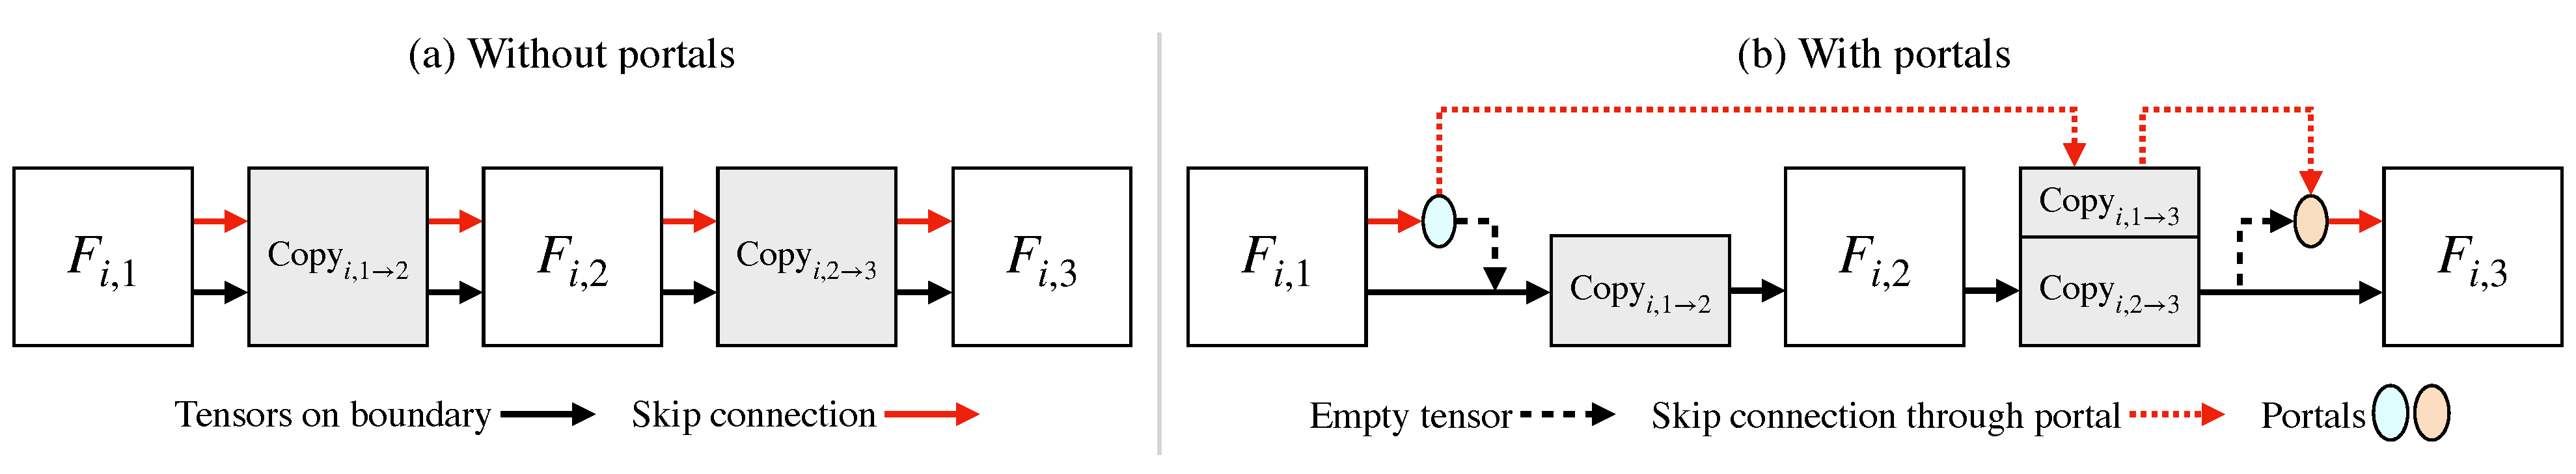
\includegraphics[width=\textwidth]{figures/portals.pdf}
    \caption{The flow of skip connection with or without portals. (a): Without portals, skipped tensor from device 1 is copied to device 2 and subsequently to device 3. (b): With portals, the tensor is directly copied to device 3. The gradient flows in the exact reverse direction in the backward pass.}
    \label{fig:portals}
\end{figure*}

In \autoref{sec:pipeline-parallelism}, we assumed that the model $f$ is composed of partitions $f^1, \cdots, f^n$ in sequence. In principle, any neural network can be represented in this form by sorting all nodes in the forward computation graph of $f$ in topological ordering. Hence, pipeline parallelism is applicable to any model.

However, consider a symptomatic case that all the partitions except the first and the last one are parallel, \emph{i.e.}, 
\[
f(y) = g^n(x^2, \cdots, x^{n-1})
\]
where $x^1 = g^1(x)$ and $x^j = g^j(x^1)$ for $j=2,\cdots,n-1$. In a sequential form, this is equivalent to $f = f^n \circ \cdots \circ f^1$ such that
\[
\begin{aligned}
    &f^n(x^1, x^2, \cdots, x^{n-1}) & &:= g^n(x^2, \cdots, x^{n-1}), \\
    &f^j(x^1, \cdots, x^{j-1}) & &:= (x^1, \cdots, x^{j-1}, f^j(x^1)) \\
\end{aligned}
\]
for $j=2,\cdots,n-1$, and $f^1 = g^1$. In this case, it is quite inefficient to use pipeline parallelism in its native form since at the boundary of device $j-1$ and $j$, the tuple $(x_i^1, \cdots, x_i^{j-1})$ must be copied instead of a single tensor $x_i^1$ which is the only required data to compute $j$th partition. 

{\torchgpipe} provides a submodule which allows users to indicate skipping tensors from which layer to which layer: \cmtt{torchgpipe.skip}. With the decorator \cmtt{@skippable}, user-defined layer can stash a tensor for later or pop a stashed one via \cmtt{yield} operator in Python without returning it. This in particular does not change the input and output signature of a layer. Hence, minimal effort is needed for adding skip connection to a preexisting sequential model. 

\subsubsection{Hiding Skip Tensors in the Graph: Portals}
\label{subsubsec:portals}

Adding skip connections into the dependency graph (\autoref{fig:pp-with-checkpointing}) is fairly straightforward. Indeed, no additional dependency would be introduced no matter how many skip connections are added, hence only the copy kernels for skip connections need extra care. In {\torchgpipe}, this is taken care by \emph{portals} consisting of three autograd functions \cmtt{PortalBlue}, \cmtt{PortalOrange}, and \cmtt{PortalCopy} sharing memory, like \cmtt{Checkpoint} and \cmtt{Recompute} in \autoref{subsubsec:checkpointing}. Each does the job of saving the skip tensor, loading the tensor, and moving the saved tensor to the skipped device, respectively (and vice versa in the backward pass). This mechanism is illustrated in \autoref{fig:portals}.